
\documentclass[aspectratio=169,10pt]{beamer}

\usetheme{default}
\setbeamertemplate{navigation symbols}{}
\setbeamertemplate{footline}{\hfill\scriptsize\insertframenumber/\inserttotalframenumber\hspace{0.8em}\vspace{0.4em}}
\setbeamertemplate{itemize items}[circle]
\setbeamertemplate{enumerate items}[default]

\usepackage[utf8]{inputenc}
\usepackage[T1]{fontenc}
\usepackage[french]{babel}
\usepackage{lmodern}
\usepackage{graphicx}
\usepackage{booktabs}
\usepackage{tabularx}
\usepackage{array}
\usepackage{amsmath}
\usepackage{xcolor}
\usepackage{hyperref}
\usepackage{tikz}
\usetikzlibrary{arrows.meta,positioning,shapes.geometric}

\definecolor{UniBlue}{RGB}{15,55,105}
\definecolor{MutedBlue}{RGB}{54,104,153}
\definecolor{DarkRed}{RGB}{170,40,40}
\definecolor{DarkGreen}{RGB}{24,112,74}
\definecolor{LightGray}{RGB}{245,247,250}

\hypersetup{
  colorlinks=true,
  urlcolor=UniBlue,
  linkcolor=UniBlue,
  pdfborder={0 0 0}
}

\setbeamercolor{normal text}{fg=black,bg=white}
\setbeamercolor{frametitle}{fg=UniBlue,bg=white}
\setbeamerfont{frametitle}{series=\bfseries,size=\large}
\setbeamerfont{title}{series=\bfseries,size=\large}
\setbeamerfont{subtitle}{size=\small}

\newcommand{\slidetitleline}{\par\vspace{-0.3em}\noindent\textcolor{UniBlue}{\rule{\linewidth}{0.7pt}}\par\vspace{0.25em}}
\newcommand{\source}[1]{\vspace{0.12em}{\tiny\color{gray}\textit{Source : #1}}}
\newcommand{\imgcaption}[1]{{\scriptsize\color{black!75}\textit{#1}}}
\newcolumntype{Y}{>{\raggedright\arraybackslash}X}
\graphicspath{{assets/}}

\title{Amélioration de l'interprétation de variants génétique par l'intégration de structure 3D de protéine et de données de dynamique moléculaire}
\subtitle{Comparaison de l'hémoglobine normale (WT) et de l'hémoglobine S (HbS)}
\author{Makwiza Mbala Judicael \and Matendo Kalaki Donat \and Mwanza Parousia Ketsia \and Mfushi Kapalay Stephen \and Luayi Kangombo Jonas}
\date{Année académique 2025--2026}

\begin{document}

% ------------------------------------------------------------
\begin{frame}[plain]
\centering
\vspace{0.1cm}

\includegraphics[width=2.35cm,keepaspectratio]{unikin_logo.png}\par
\vspace{0.25cm}
{\scriptsize UNIVERSITÉ DE KINSHASA\par}
{\scriptsize Faculté des Sciences et Technologies -- Département de Mathématiques, Statistique et Informatique\par}
\vspace{0.38cm}
{\color{UniBlue}\bfseries\fontsize{15.5}{18.5}\selectfont Amélioration de l'interprétation de variants génétique par l'intégration de structure 3D de protéine et de données de dynamique moléculaire\par}
\vspace{0.17cm}
{\small\bfseries Comparaison de l'hémoglobine normale (WT) et de l'hémoglobine S (HbS)\par}
\vspace{0.35cm}
{\normalsize Travail Pratique de Programmation et algorithmes pour la bioinformatique\par}
\vspace{0.35cm}
{\footnotesize\textbf{Membres du groupe :} Makwiza Mbala Judicael, Matendo Kalaki Donat, Mwanza Parousia Ketsia, Mfushi Kapalay Stephen, Luayi Kangombo Jonas\par}
\vspace{0.18cm}
{\footnotesize\textbf{Titulaire :} Professeur Christian D. BOPE \quad -- \quad \textbf{Doctorant :} Keph Makoy\par}
\vfill
{\footnotesize Dépôt GitHub : \href{https://github.com/JudicaelMAKWIZA/HBB_MD_Interpretation}{\texttt{github.com/JudicaelMAKWIZA/HBB\_MD\_Interpretation}}\par}
\end{frame}

% ------------------------------------------------------------
\begin{frame}{Introduction : hémoglobine, HbS et contexte clinique}
\slidetitleline
\begin{columns}[T,totalwidth=\textwidth]
\begin{column}{0.52\textwidth}
\small
L'hémoglobine adulte est une protéine tétramérique \(\alpha_2\beta_2\) qui transporte l'oxygène grâce à quatre groupes hème. Le gène \textbf{HBB} code la chaîne \(\beta\).

\vspace{0.45em}
Le variant \textbf{HBB c.20A>T} conduit à l'hémoglobine S (HbS). Dans la chaîne \(\beta\) mature, il est généralement noté \textbf{\(\beta\)Glu6Val} : un glutamate chargé est remplacé par une valine hydrophobe.

\vspace{0.45em}
Cette modification locale favorise, en condition désoxygénée, des contacts entre molécules HbS et la polymérisation responsable de la drépanocytose. Notre travail étudie donc l'effet structural du variant dans un tétramère isolé.
\end{column}
\begin{column}{0.44\textwidth}
\centering
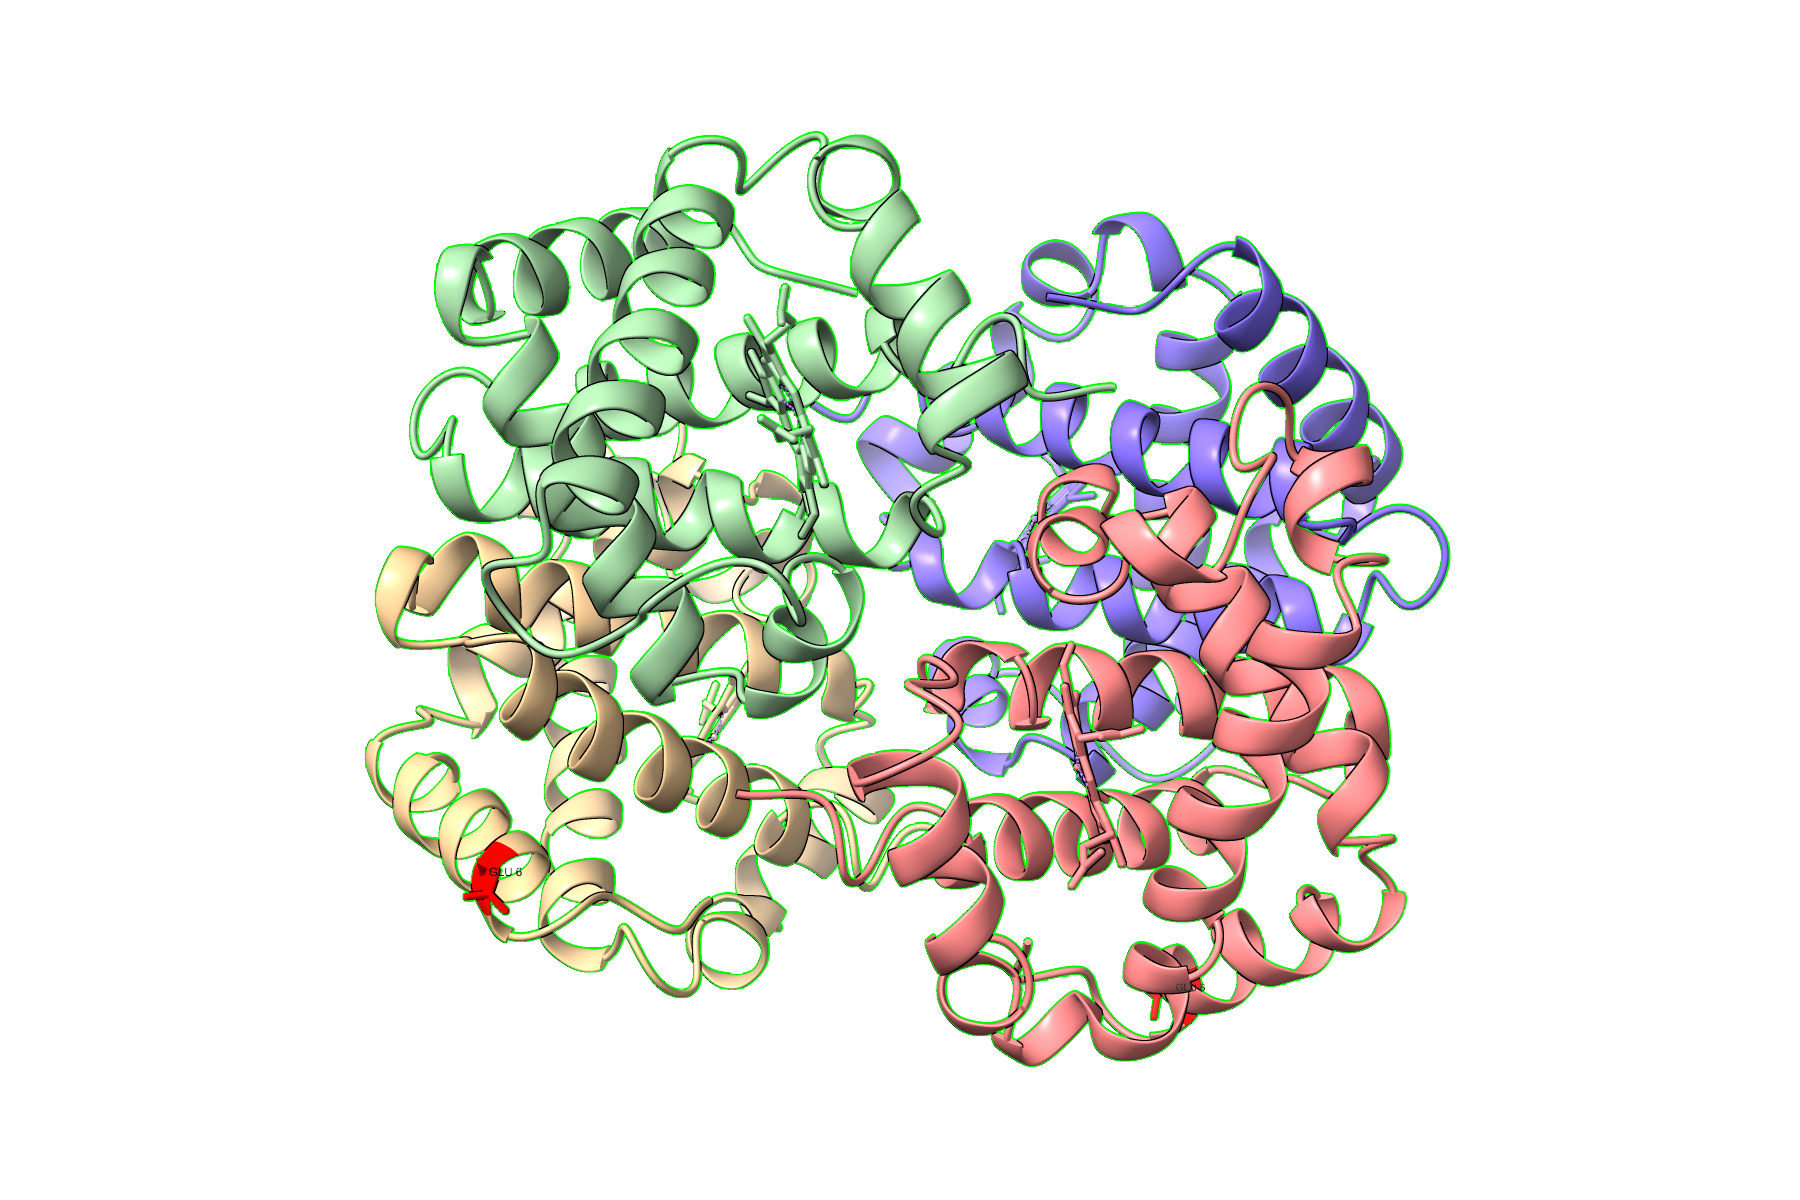
\includegraphics[width=0.98\linewidth,height=0.56\textheight,keepaspectratio]{WT_global.png}\par
\imgcaption{Architecture complète de l'hémoglobine : quatre chaînes globines et quatre hèmes.}\par
\source{Visualisation ChimeraX générée dans le projet à partir de la structure PDB 2DN2.}
\end{column}
\end{columns}
\vspace{0.3em}
{\scriptsize Les détails complets du protocole, les scripts, les fichiers MDP, les figures et les résultats sont documentés dans le \href{https://github.com/JudicaelMAKWIZA/HBB_MD_Interpretation}{README du dépôt GitHub}.}
\end{frame}

% ------------------------------------------------------------
\begin{frame}[shrink=5]{Problématique, hypothèse et objectifs}
\slidetitleline
\small
\textbf{Problématique.} Dans quelle mesure l'intégration de l'annotation du variant, des structures 3D de protéines et des données de dynamique moléculaire permet-elle de mieux interpréter l'impact structural du variant \textbf{HBB \(\beta\)Glu6Val} ?

\vspace{0.5em}
\textbf{Hypothèse.} La substitution Glu \(\rightarrow\) Val peut modifier localement la dynamique et la compacité de l'hémoglobine. Toutefois, dans un tétramère isolé, ces différences devraient rester modestes si l'effet pathogène majeur dépend surtout des interactions \textbf{intermoléculaires} entre molécules HbS.

\vspace{0.6em}
\textbf{Objectifs réalisés.}
\begin{enumerate}\footnotesize
  \item Documenter le variant HBB étudié et son contexte clinique.
  \item Comparer les structures 3D de l'hémoglobine normale (WT) et de l'hémoglobine S (HbS).
  \item Construire deux modèles moléculaires comparables et validés sous GROMACS.
  \item Produire une dynamique moléculaire pilote de 1 ns par modèle.
  \item Interpréter RMSD, RMSF, rayon de giration et visualisations ChimeraX.
\end{enumerate}
\end{frame}

% ------------------------------------------------------------
\begin{frame}{Méthode : pipeline de l'analyse}
\slidetitleline
\small
\begin{center}
\begin{tikzpicture}[scale=0.82,transform shape,
node distance=0.30cm,
mystep/.style={draw=UniBlue,rounded corners=1.5pt,minimum height=0.75cm,text width=2.05cm,align=center,font=\scriptsize},
arr/.style={-{Latex[length=2.1mm]},thick,draw=UniBlue}]
\node[mystep] (a) {Variant HBB\\ClinVar};
\node[mystep,right=of a] (b) {Structures PDB\\2DN2 / 2HBS};
\node[mystep,right=of b] (c) {Préparation\\chaînes A--D + HEM};
\node[mystep,right=of c] (d) {Validation\\topologie + ions};
\node[mystep,right=of d] (e) {MD\\EM, NVT, NPT, 1 ns};
\node[mystep,right=of e] (f) {Analyses\\RMSD, RMSF, Rg};
\draw[arr] (a)--(b); \draw[arr] (b)--(c); \draw[arr] (c)--(d); \draw[arr] (d)--(e); \draw[arr] (e)--(f);
\end{tikzpicture}
\end{center}

\vspace{0.35em}
\begin{columns}[T,totalwidth=\textwidth]
\begin{column}{0.49\textwidth}
\textbf{Préparation des structures}\par
\footnotesize
Les structures expérimentales ont été nettoyées pour conserver les chaînes A--D et les quatre hèmes. Les histidines proximales et les liaisons His--Fe ont été harmonisées afin de comparer WT et HbS dans des conditions cohérentes.
\end{column}
\begin{column}{0.49\textwidth}
\textbf{Simulation et analyse}\par
\footnotesize
Après minimisation, NVT et NPT, une production pilote de 1 ns a été réalisée. Les métriques retenues répondent à trois questions : stabilité globale (RMSD), mobilité locale (RMSF) et compacité (Rg).
\end{column}
\end{columns}
\vspace{0.3em}
\source{GROMACS 2023.3, UCSF ChimeraX, scripts disponibles dans le dépôt GitHub.}
\end{frame}

% ------------------------------------------------------------
\begin{frame}{Préparation et validation}
\slidetitleline
\small
Cette étape vise à rendre les deux \textbf{modèles moléculaires} WT et HbS directement comparables avant la dynamique : même type de boîte, solvant, concentration saline, traitement des hèmes et protocole de validation.

\vspace{0.55em}
\begin{columns}[T,totalwidth=\textwidth]
\begin{column}{0.50\textwidth}
\textbf{Choix techniques principaux}\par
\footnotesize
\begin{itemize}
  \item GROMACS 2023.3 ; champ de force \texttt{GROMOS54A7\_hbb}.
  \item Eau SPC ; boîte dodécaédrique commune de 682,654 nm\(^3\).
  \item NaCl 0,15 M et neutralisation de la charge totale.
  \item Quatre hèmes conservés ; liaisons proximales His--Fe validées.
\end{itemize}
\end{column}
\begin{column}{0.48\textwidth}
\textbf{Contrôles effectués}\par
\footnotesize
\begin{itemize}
  \item WT et HbS : 574 résidus protéiques et 4 hèmes.
  \item Absence d'erreur bonded après correctif local documenté.
  \item Aucun \textit{LINCS warning} sur NVT, NPT et production.
  \item Un seul avertissement GROMOS connu accepté dans \texttt{grompp}.
\end{itemize}
\end{column}
\end{columns}

\vspace{0.45em}
\centering
\scriptsize
\begin{tabular}{lccc}
\toprule
Modèle & Atomes après ions & Eaux & Ions ajoutés \\
\midrule
WT & 65 571 & 19 879 & 68 Na\(^+\), 62 Cl\(^-\) \\
HbS & 65 415 & 19 829 & 66 Na\(^+\), 62 Cl\(^-\) \\
\bottomrule
\end{tabular}
\end{frame}

% ------------------------------------------------------------
\begin{frame}{Équilibration et stabilité thermodynamique}
\slidetitleline
\small
\textbf{Rôle de l'équilibration.} La minimisation élimine les contacts défavorables. Le NVT stabilise la température autour de 300 K. Le NPT stabilise pression et densité. Une étape NPT libre précède la production pour observer la dynamique propre de la protéine.

\vspace{0.5em}
\begin{columns}[T,totalwidth=\textwidth]
\begin{column}{0.41\textwidth}
\footnotesize
\textbf{Protocole}\par
\begin{tabular}{ll}
Minimisation & steepest descent \\
NVT & 100 ps, 300 K \\
NPT contraint & 300 ps \\
NPT libre & 200 ps \\
Production & 1 ns par modèle \\
\end{tabular}

\vspace{0.5em}
\textbf{Minimisation}\par
WT : Fmax = 959,85 kJ mol\(^{-1}\) nm\(^{-1}\)\par
HbS : Fmax = 943,06 kJ mol\(^{-1}\) nm\(^{-1}\)
\end{column}
\begin{column}{0.56\textwidth}
\centering
\scriptsize
\begin{tabular}{lcc}
\toprule
Métrique de production & WT & HbS \\
\midrule
Température & 299,94 \(\pm\) 1,26 K & 299,88 \(\pm\) 1,31 K \\
Pression & 0,32 \(\pm\) 106,81 bar & -0,01 \(\pm\) 102,22 bar \\
Densité & 1017,59 \(\pm\) 1,90 kg/m\(^3\) & 1016,93 \(\pm\) 1,87 kg/m\(^3\) \\
\bottomrule
\end{tabular}
\vspace{0.4em}

\imgcaption{Les températures et densités restent stables et très proches. Les fluctuations de pression sont importantes, comme attendu à cette échelle atomistique, mais les moyennes restent proches de la cible.}
\end{column}
\end{columns}
\end{frame}

% ------------------------------------------------------------
\begin{frame}{Résultats globaux : stabilité et compacité}
\slidetitleline
\begin{columns}[T,totalwidth=\textwidth]
\begin{column}{0.50\textwidth}
\centering
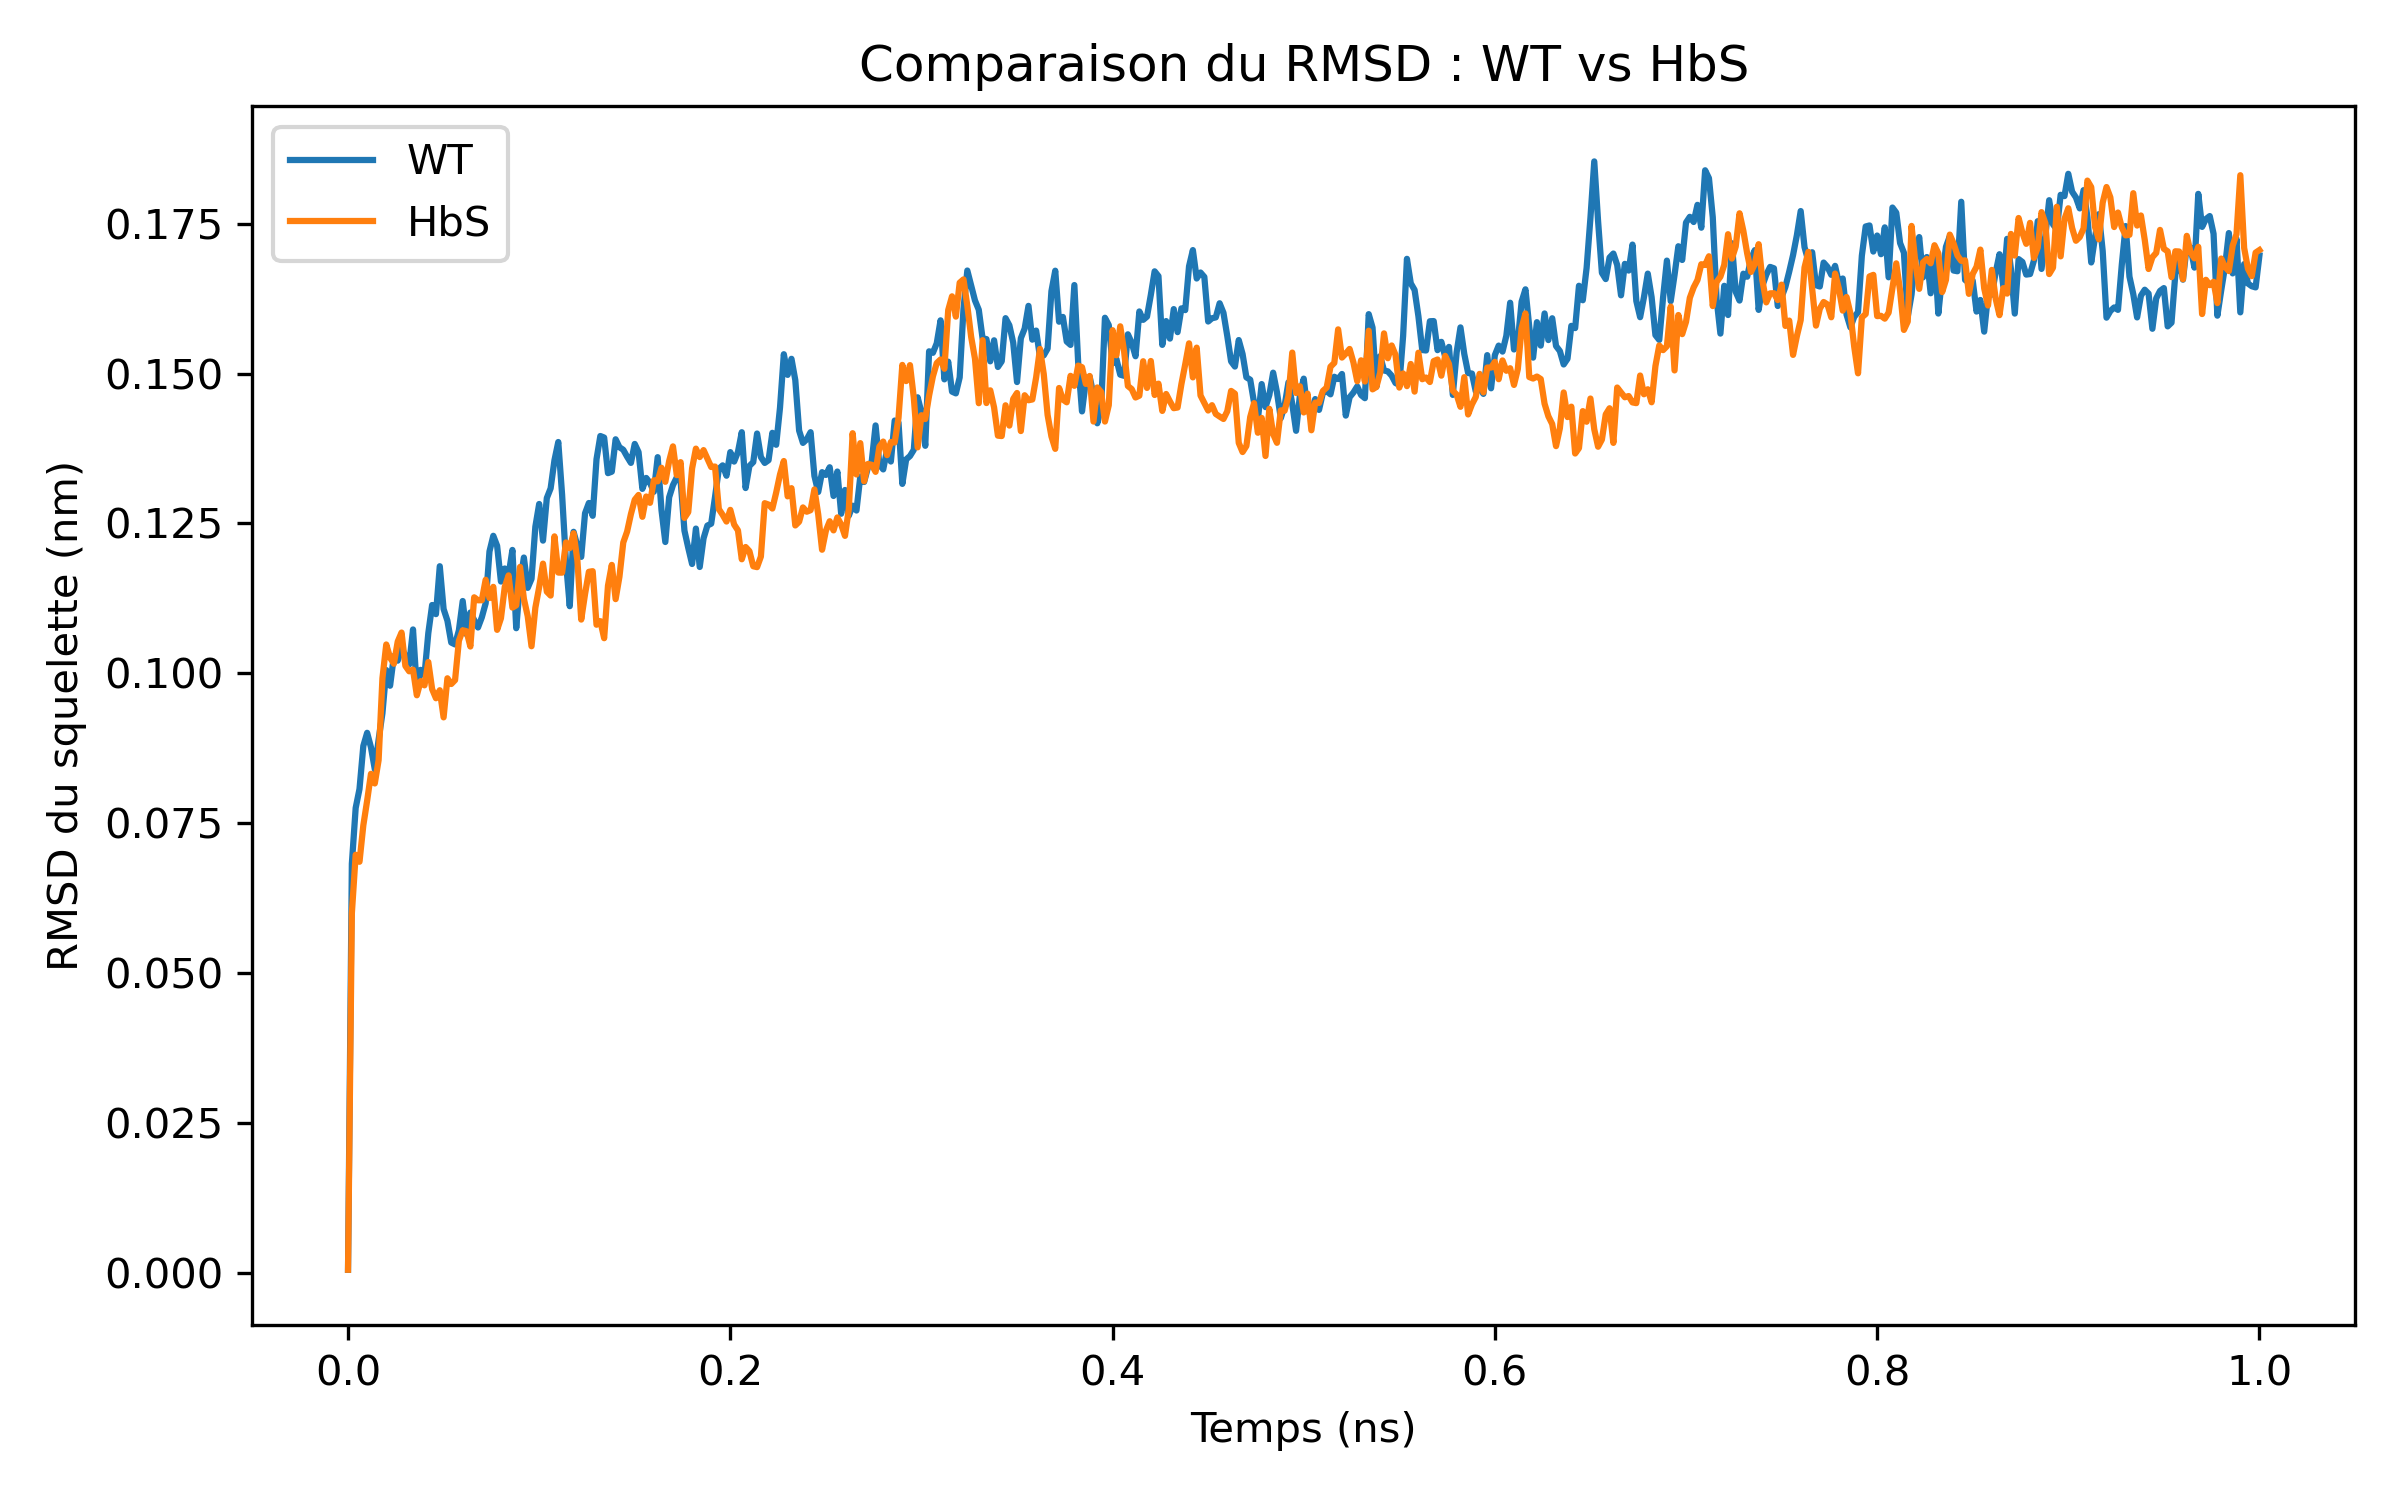
\includegraphics[width=0.96\linewidth,height=0.50\textheight,keepaspectratio]{rmsd_WT_vs_HbS.png}\par
\imgcaption{RMSD du squelette : les deux modèles restent stables et très proches sur 1 ns.}\par
\source{Analyse GROMACS, production 1 ns, ajustement PBC corrigé.}
\end{column}
\begin{column}{0.50\textwidth}
\centering
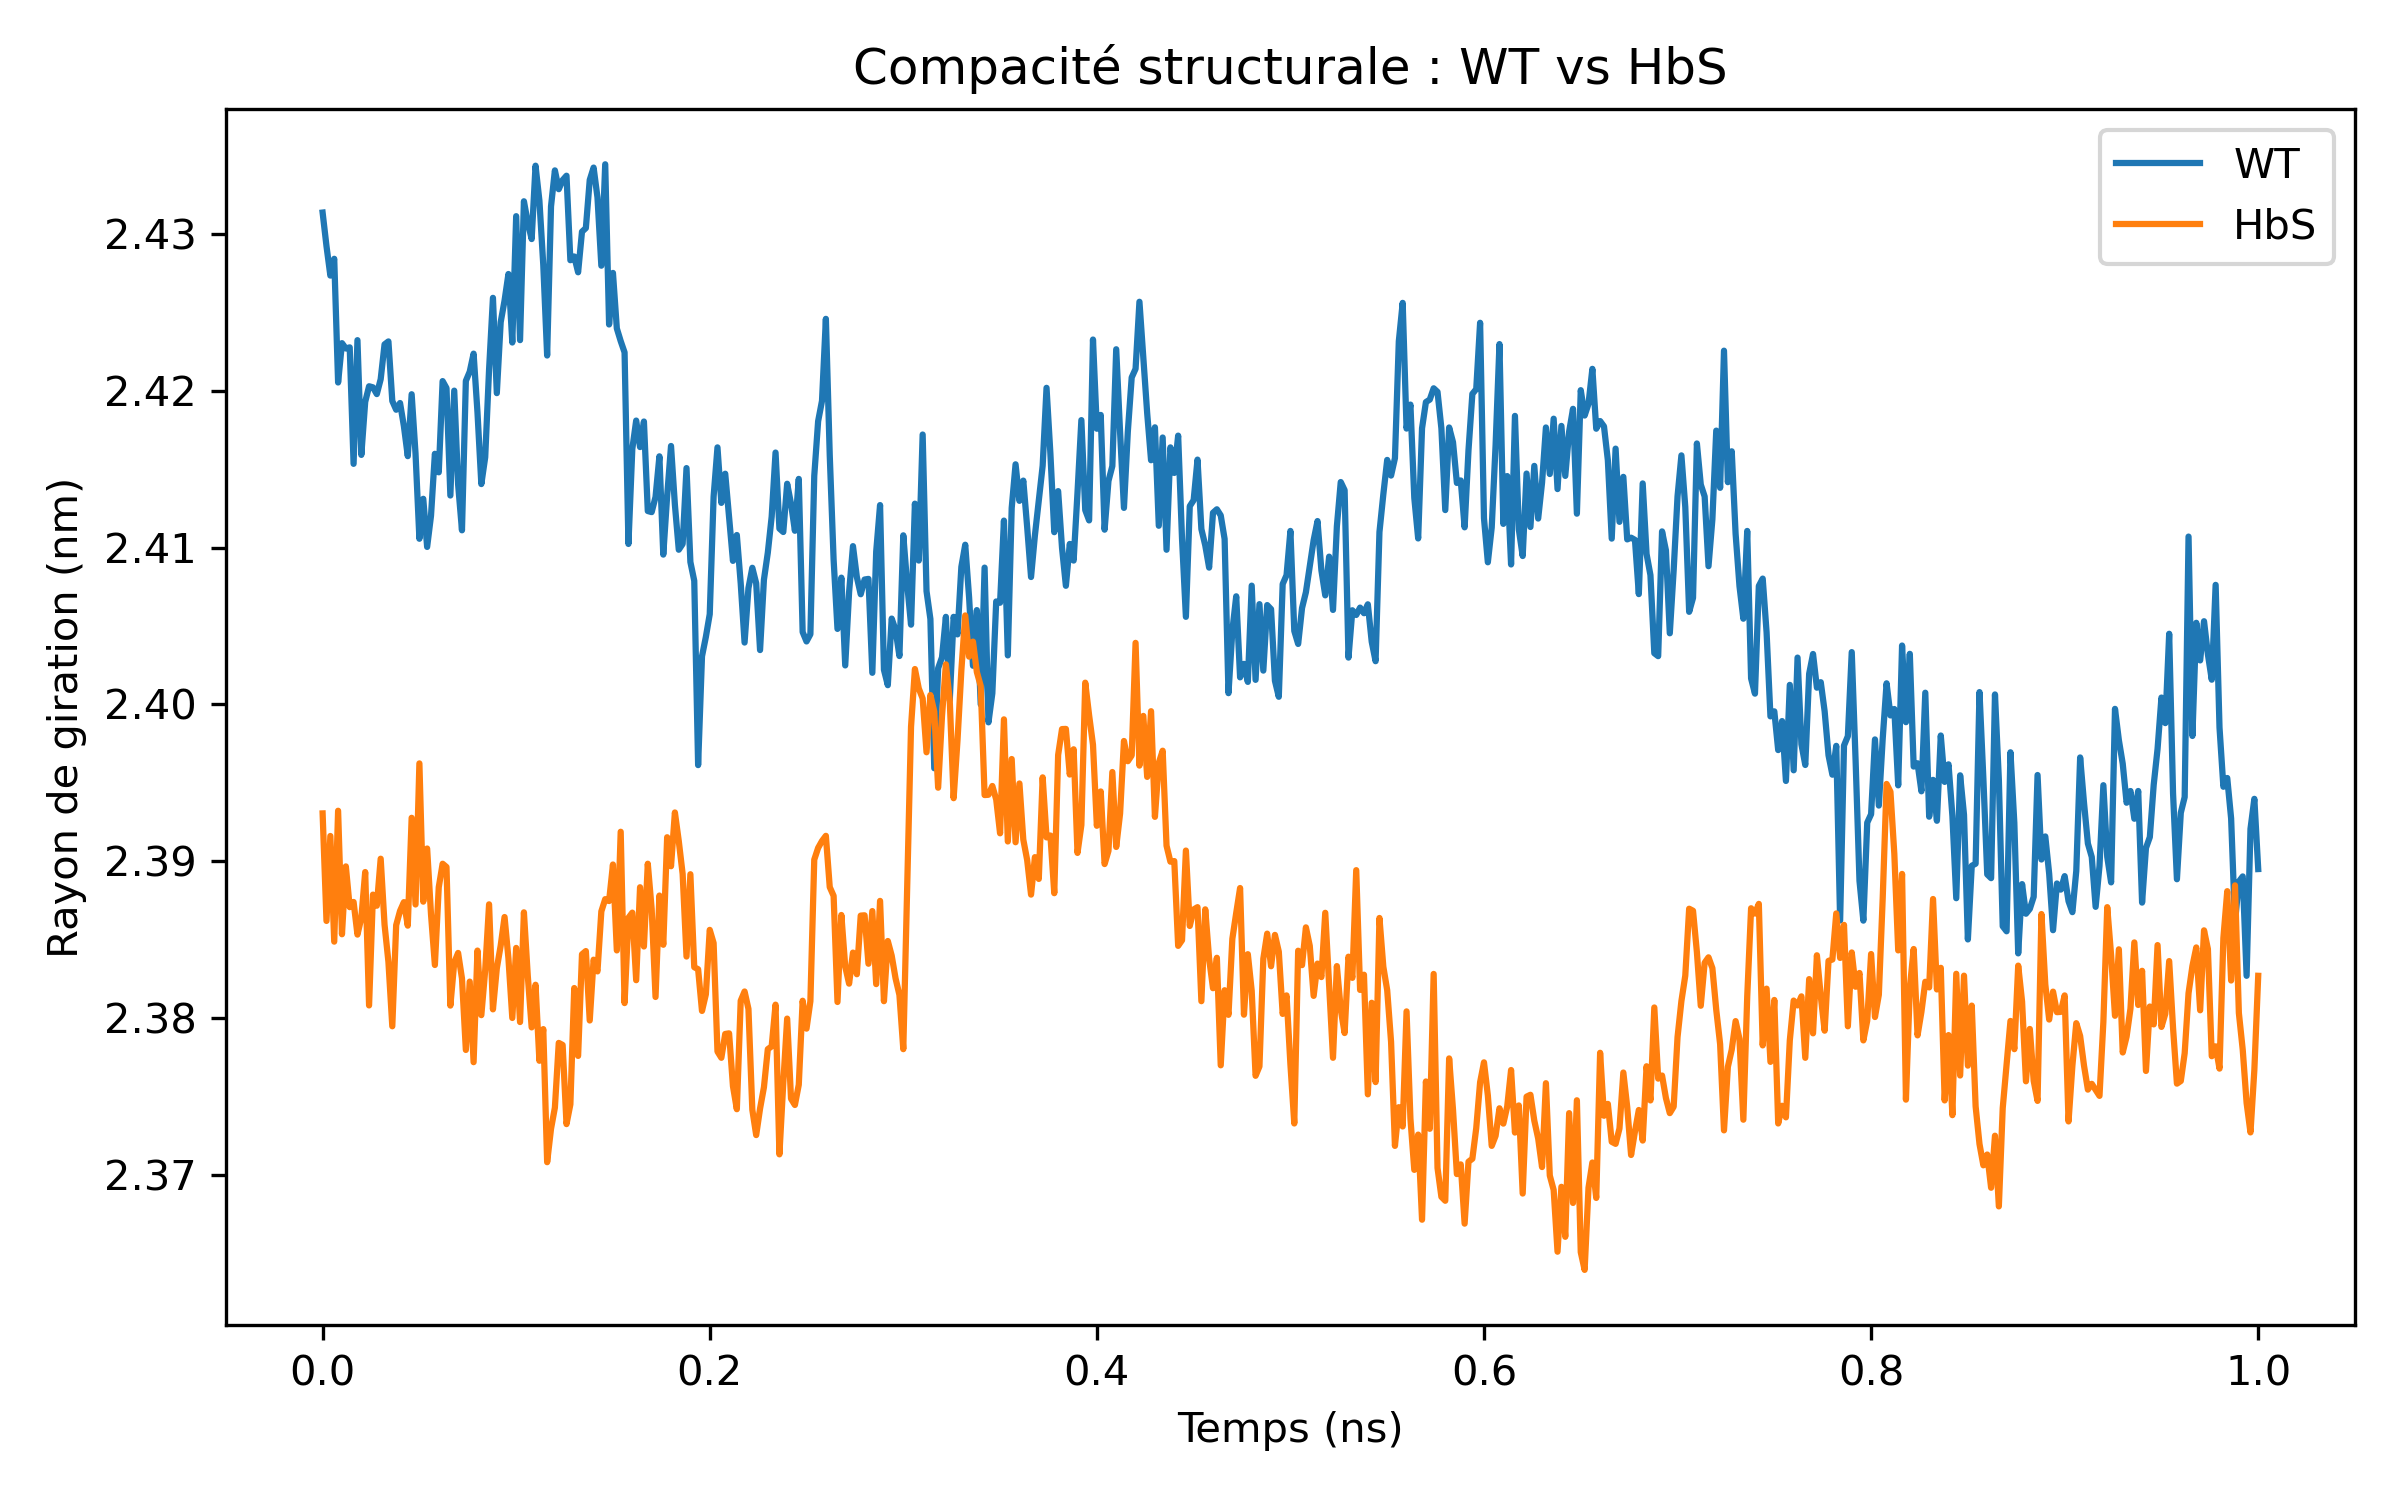
\includegraphics[width=0.96\linewidth,height=0.50\textheight,keepaspectratio]{rg_WT_vs_HbS.png}\par
\imgcaption{Rayon de giration : HbS est légèrement plus compacte, avec une différence faible.}\par
\source{Analyse GROMACS, production 1 ns.}
\end{column}
\end{columns}

\vspace{0.35em}
\centering
\scriptsize
\begin{tabular}{lccc}
\toprule
Métrique & WT & HbS & \(\Delta\) HbS--WT \\
\midrule
RMSD moyen & 0,1581 \(\pm\) 0,0122 nm & 0,1533 \(\pm\) 0,0140 nm & -0,0048 nm \\
Rg moyen & 2,4059 \(\pm\) 0,0096 nm & 2,3821 \(\pm\) 0,0083 nm & -0,0238 nm \\
\bottomrule
\end{tabular}
\end{frame}

% ------------------------------------------------------------
\begin{frame}{Résultats locaux : flexibilité autour de \(\beta\)6}
\slidetitleline
\begin{columns}[T,totalwidth=\textwidth]
\begin{column}{0.49\textwidth}
\centering
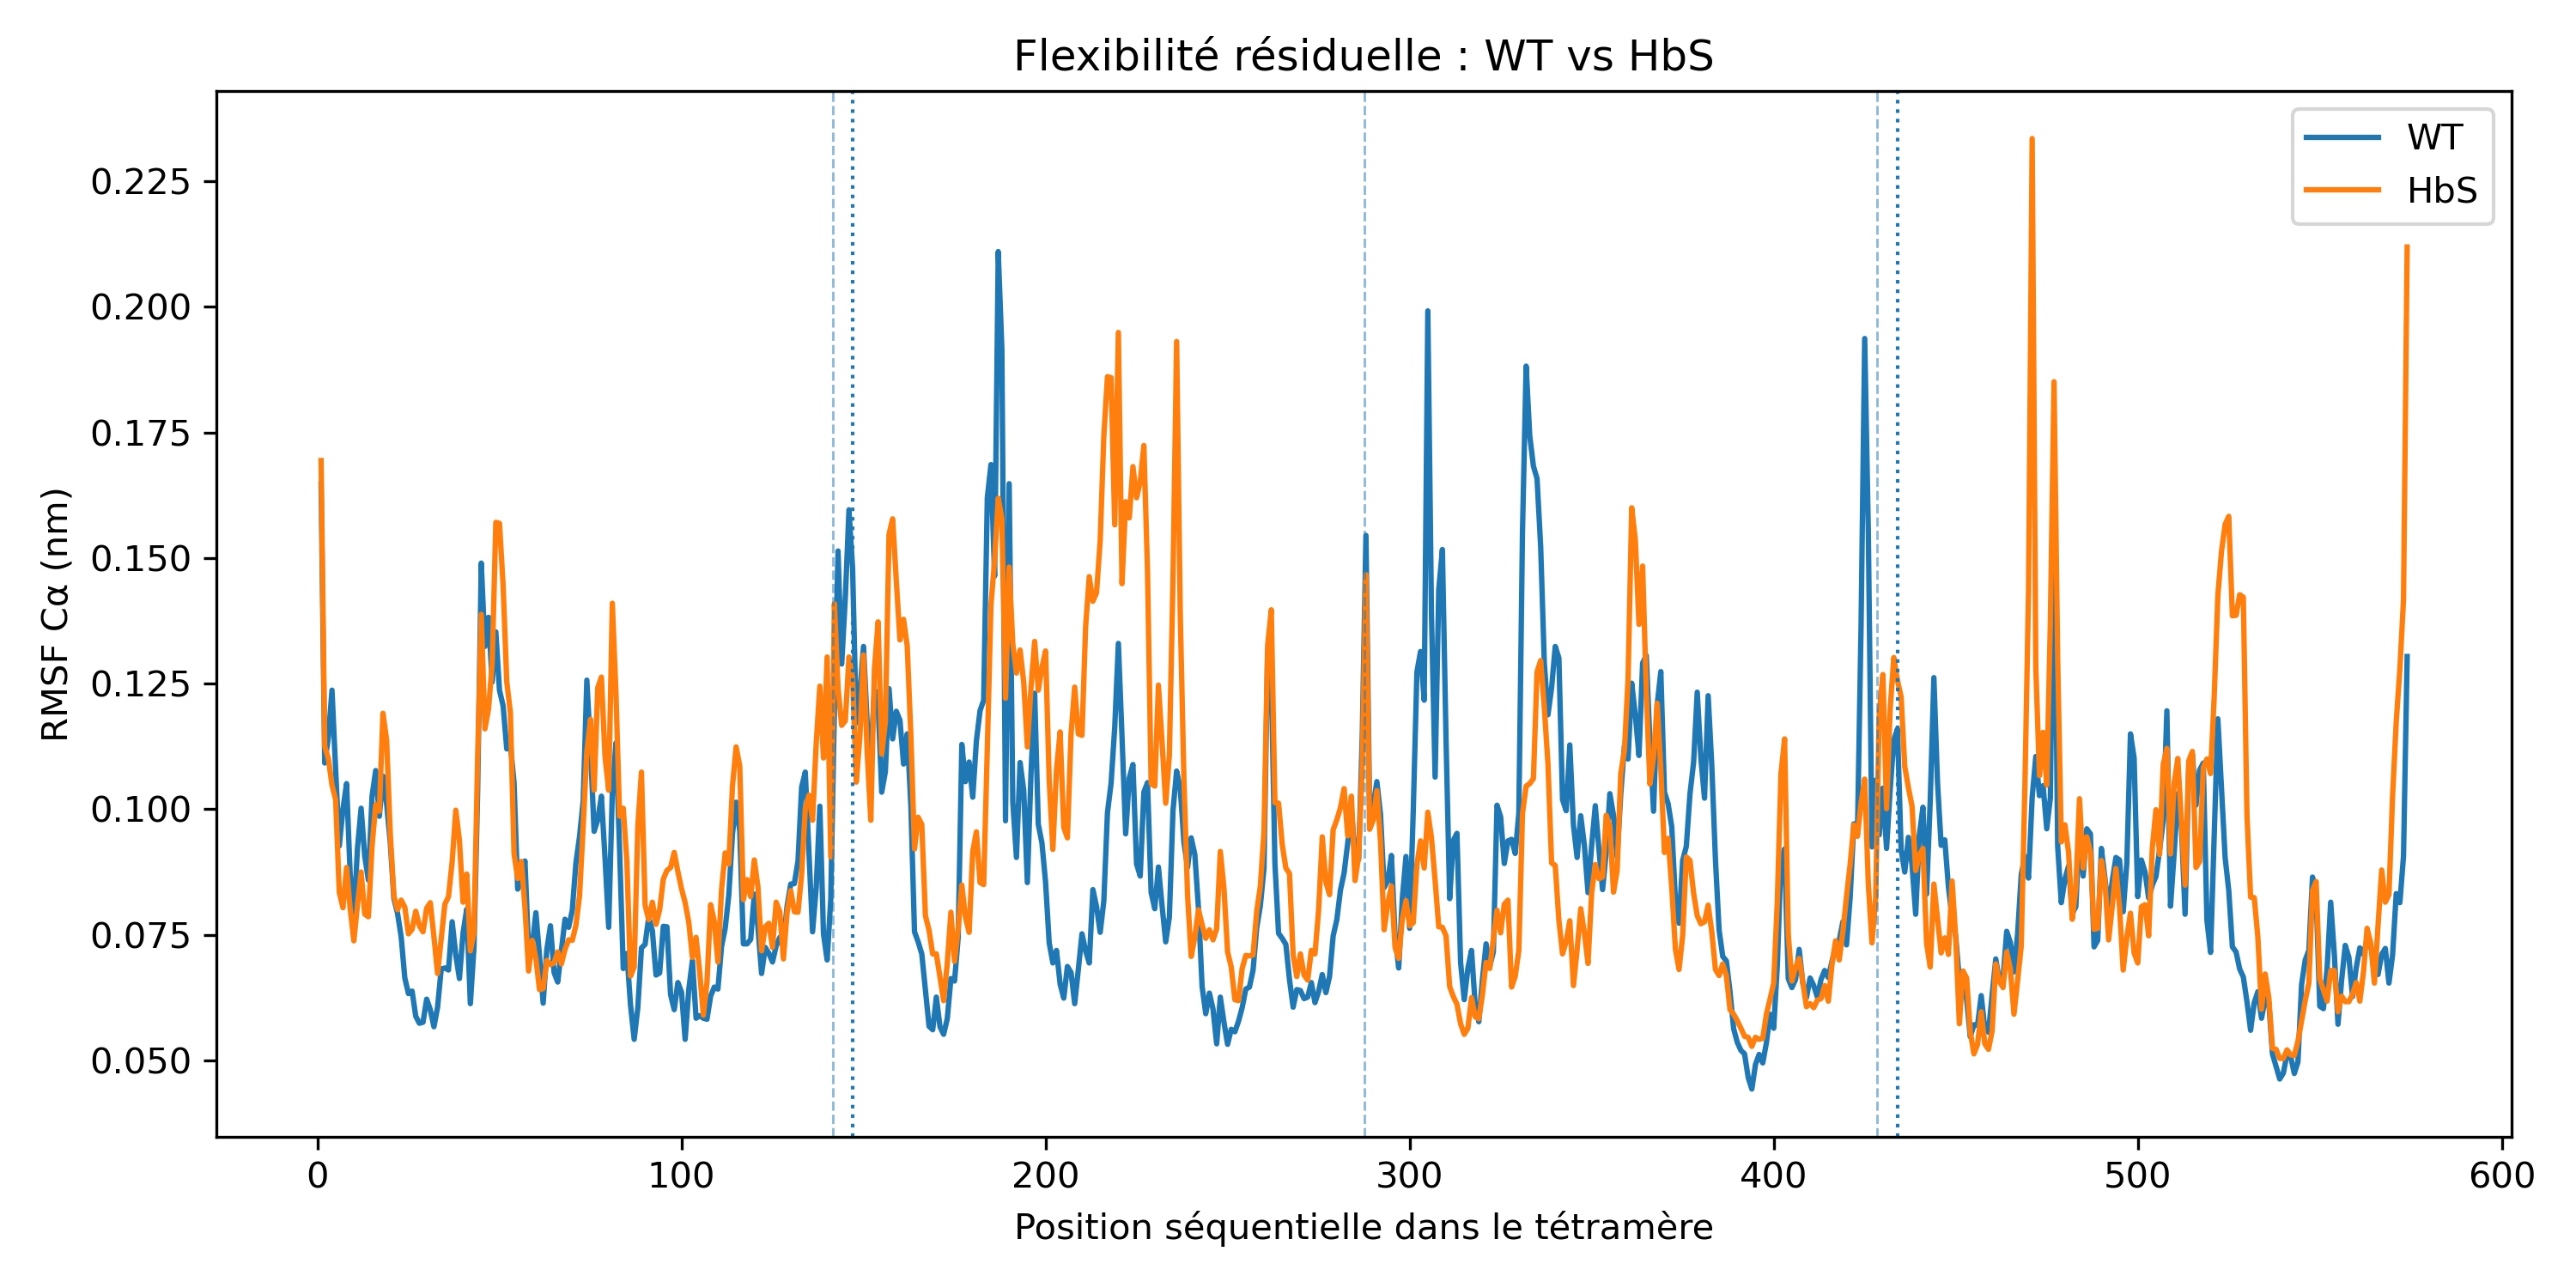
\includegraphics[width=0.98\linewidth,height=0.40\textheight,keepaspectratio]{rmsf_WT_vs_HbS.png}\par
\imgcaption{RMSF C\(\alpha\) par position dans le tétramère. Les lignes verticales indiquent les limites de chaînes et les positions \(\beta\)6.}\par
\source{Analyse GROMACS sur 200--1000 ps.}
\end{column}
\begin{column}{0.49\textwidth}
\centering
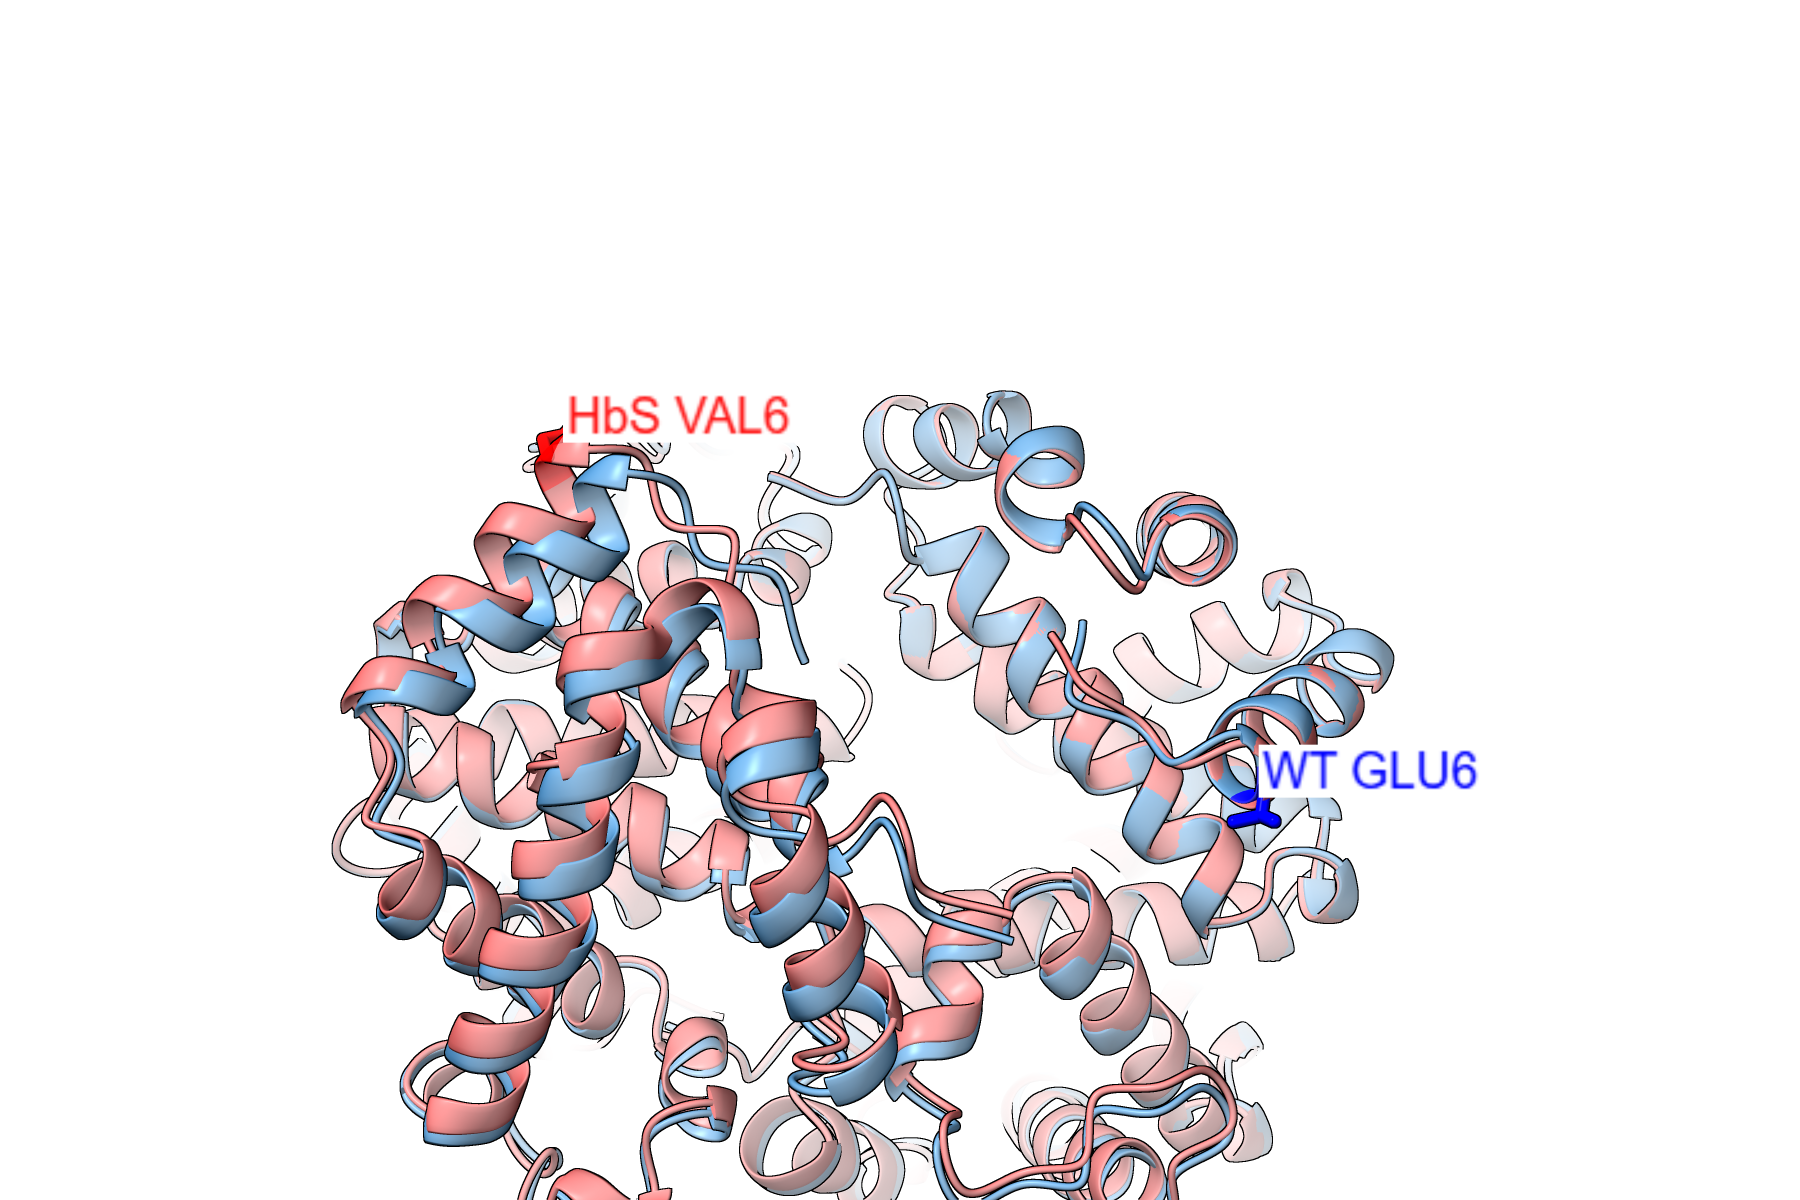
\includegraphics[width=0.98\linewidth,height=0.40\textheight,keepaspectratio]{WT_vs_HbS_overlay.png}\par
\imgcaption{Superposition locale WT/HbS : GLU6 et VAL6 sont mis en évidence sur la chaîne \(\beta\).}\par
\source{UCSF ChimeraX, structures PDB 2DN2 et 2HBS préparées dans le projet.}
\end{column}
\end{columns}

\vspace{0.25em}
\centering
\scriptsize
\begin{tabular}{lccc}
\toprule
Métrique locale & WT & HbS & \(\Delta\) HbS--WT \\
\midrule
RMSF C\(\alpha\) moyen & 0,0882 nm & 0,0932 nm & +0,0050 nm \\
RMSF \(\beta\)6 moyen & 0,1320 nm & 0,1258 nm & -0,0061 nm \\
Voisinage \(\beta\)6 \(\pm\)5 & 0,1144 nm & 0,1164 nm & +0,0020 nm \\
\bottomrule
\end{tabular}

\vspace{0.25em}
{\footnotesize Les différences locales existent mais restent faibles ; la position \(\beta\)6 ne montre pas une mobilité fortement accrue dans HbS.}
\end{frame}

% ------------------------------------------------------------
\begin{frame}{Interprétation biologique et limites}
\slidetitleline
\small
\textbf{Interprétation principale.}\par
Sur cette simulation pilote de 1 ns, WT et HbS conservent une stabilité globale comparable. La mutation \(\beta\)Glu6Val ne provoque pas de déstabilisation majeure du tétramère isolé. Cette observation est cohérente avec un mécanisme pathogène dominé par des contacts \textbf{intermoléculaires} entre molécules HbS et par la polymérisation, plutôt que par l'effondrement d'un tétramère unique.

\vspace{0.6em}
\textbf{Limites à retenir.}\par
\footnotesize
\begin{itemize}
  \item La production de 1 ns est courte : les résultats doivent être interprétés comme exploratoires.
  \item WT et HbS proviennent de deux structures cristallographiques différentes ; les différences ne peuvent pas être attribuées exclusivement à la mutation.
  \item Le modèle simule un tétramère isolé ; il ne reproduit pas la polymérisation de nombreuses molécules HbS.
  \item Pour aller plus loin : productions plus longues, réplicats indépendants et simulations de contacts intermoléculaires HbS.
\end{itemize}

\vspace{0.4em}
\textbf{Conclusion.} L'intégration structure 3D + dynamique moléculaire améliore l'interprétation du variant en distinguant un effet local mesurable d'une déstabilisation globale non observée dans ce protocole pilote.
\end{frame}

% ------------------------------------------------------------
\begin{frame}[shrink=4]{Reproductibilité, remerciements et références}
\slidetitleline
\small
\textbf{Dépôt GitHub cliquable.}\par
\href{https://github.com/JudicaelMAKWIZA/HBB_MD_Interpretation}{\texttt{github.com/JudicaelMAKWIZA/HBB\_MD\_Interpretation}}

\vspace{0.45em}
\textbf{Utilisation du README.}\par
\footnotesize
Pour garder les diapositives lisibles, le détail reproductible est placé dans le README du dépôt : commandes, scripts, fichiers MDP, figures, résultats, limites et instructions de reproduction.

\vspace{0.45em}
\textbf{Remerciements.}\par
\footnotesize
Nous remercions le \textbf{Professeur Christian D. BOPE} pour le cours et l'encadrement pédagogique, ainsi que le \textbf{Doctorant Keph Makoy} pour l'accompagnement du Travail Pratique.

\vspace{0.45em}
\textbf{Références essentielles.}\par
\scriptsize
\begin{thebibliography}{9}
\bibitem{course} Christian D. BOPE. \textit{Programmation et algorithmes pour la bioinformatique - Notes de cours détaillées}. Université de Kinshasa, 2025--2026.
\bibitem{subject} Document de sujets du Travail Pratique de Bioinformatique M2 : consignes de présentation et dépôt GitHub.
\bibitem{rcsb} RCSB PDB : structures 2DN2 (hémoglobine WT) et 2HBS (désoxyhémoglobine S).
\bibitem{clinvar} NCBI ClinVar : HBB c.20A>T / HbS / rs334.
\bibitem{gromacs} Abraham et al., \textit{GROMACS}, SoftwareX, 2015 ; manuel GROMACS 2023.3.
\bibitem{chimerax} Pettersen et al., \textit{UCSF ChimeraX}, Protein Science, 2021.
\end{thebibliography}
\end{frame}

\end{document}
